\documentclass[a4paper,12pt]{scrartcl}
\usepackage[utf8x]{inputenc}
\usepackage[T1]{fontenc} % avec T1 comme option  d'encodage c'est ben mieux, surtout pour taper du français.
%\usepackage{lmodern,textcomp} % fortement conseillé pour les pdf. On peut mettre autre chose : kpfonts, fourier,...
\usepackage[french]{babel} %Sans ça les guillemets, amarchpo
\usepackage{amsmath}
\usepackage{multicol}
\usepackage{amssymb}
\usepackage{tkz-tab}
\usepackage{exercice_sheet}

%\trait
%\section*{}
%\exo{}
%\question{}
%\subquestion{}

\date{}


% Title Page
\title{Fiche d'exercices \og Techniques de dérivation \fg{}, corrigé}

\author{Mathématiques}

\begin{document}

\maketitle

\exo{Déterminer les dérivées $f'(x)$ des fonctions $f$ définies par:}

\question{}
$f'(x) = 3 \, x^{2} + 6 \, x - 5$

\question{}
$f'(x) = \frac{3}{x} + 5 \, e^{x}$

\question{}
$f'(x) = 3 \, x^{2} - \frac{4}{x^{2}} - 5$

\question{}
$f'(x) = \frac{1}{2 \, \sqrt{x}} + 2$

Pour les exercices 2 à 4, il s'agit de reconnaître les formes vues en cours ($f = u \times v$, $f = \frac{u}{v}$, $f = u\circ v$ etc.)

\exo{Même consigne}

\question{}
Ici, on reconnaît la forme $f(x) = 2 \times e^{u(x)}$ avec $u(x) = -0.4x+3$

$f'(x) = 2 \times (-0.4) e^{-0.4x+3} = -0.8e^{-0.4x+3}$

\question{}
$f'(x) = \frac{20}{4x+1}$

\question{}
$f'(x) = 6(2x+1)^2$

\question{}
$f'(x) = \frac{2x}{x^2+1} + 2 e^{2x+1}$

\exo{Idem}

\question{}
$5 \, x^{2} {\left(3 \, \ln\left(x\right) + 1\right)}$

\question{}
$f'(x) = {\left(x + 2\right)} x e^{x}$

\question{}
$f'(x) = x {\left(2 \, \ln\left(x\right) + 1\right)}$

\question{}
$f'(x) = \frac{\frac{1}{x}(3 \, x - 1) - 3 \, \ln\left(x\right)}{{\left(3 \, x - 1\right)}^{2}}$

\question{}
$-3 e^{x}\frac{{\left(2 \, x - 1\right)} }{{\left(2 \, x + 1\right)}^{2}}$

\question{}
$f'(x) = \frac{-5}{x \ln^2(x)}$

\question{}
$f'(x) = \frac{-4}{(4x+1)^2}$

\exo{Encore}

\question{}
$f'(x) = 2 \, {\left(6 \, x + 5\right)} {\left(3 \, x + 1\right)} e^{4 \, x}$

\question{}
$f'(x) = \frac{-8 \, e^{0.2 \, x}}{{\left(10 \, e^{0.2 \, x} + 1\right)}^{2}}$

\question{}
On remarque que $\ln \left( e^{2x} \right) = 2x$. On obtient donc:
$f'(x) = 2$

\exo{}
Soit $f$ la fonction définie par $f(x) = \dfrac{4}{x} - 1$ pour $x \in \left[ \dfrac{1}{2} ; 5\right]$. Sa représentation graphique est la courbe $\mathcal{C}_f$ donnée ci-dessous:

\begin{figure}[h]
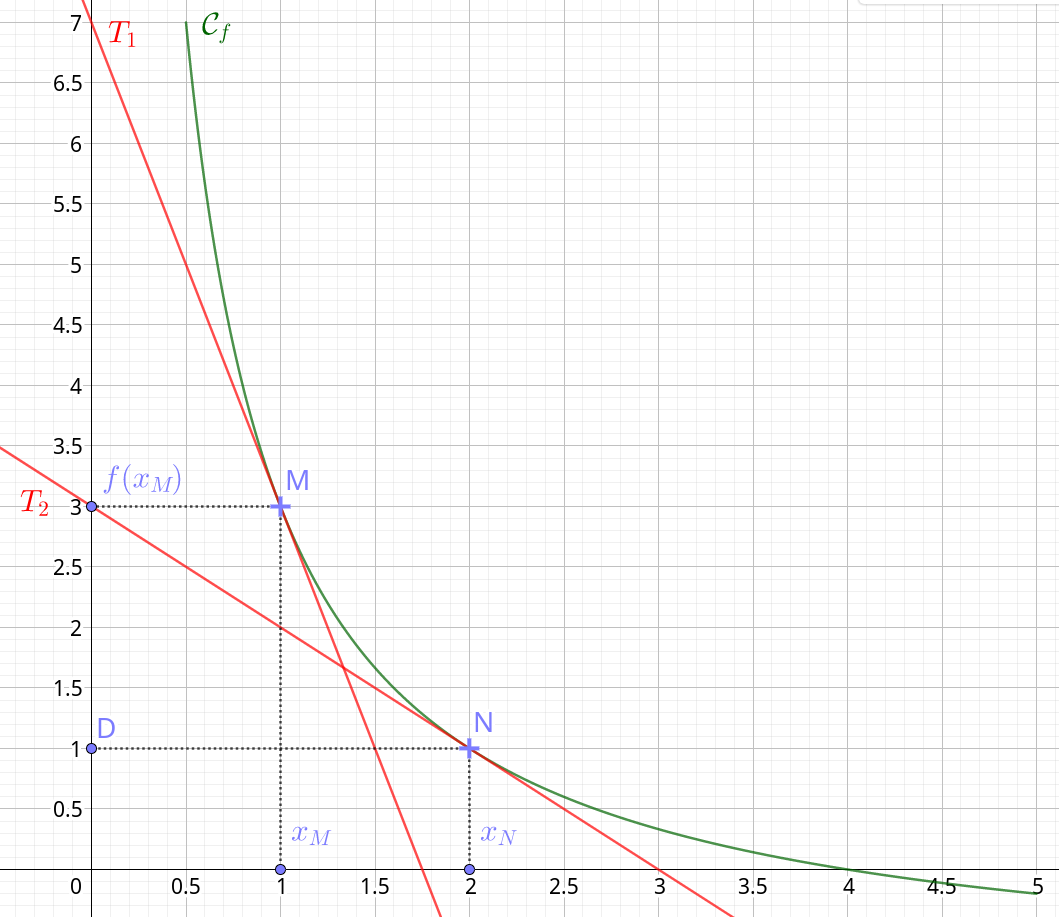
\includegraphics[width=.9\textwidth]{pics/graph1.png}
\caption{Graphe complété}
\label{graphe1}
\end{figure}

\question{}
$f'(x) = \dfrac{-4}{x^{2}}$

\question{Coordonnées des points $M$ et $N$.}

\littlestar{Point $M$} $M$ a pour coordonnées $(x_M ; f(x_M))$. 

$f(x_M) = f(1) = \frac{4}{1} - 1 = 3$

$M$ a donc pour coordonnées $(1;3)$.

\littlestar{Point $N$} $N$ a pour coordonnées $(x_N ; f(x_N))$. 

$f(x_N) = f(2) = \frac{4}{2} - 1 = 1$

$N$ a donc pour coordonnées $(2;1)$.



\question{}

\littlestar{En $x = 1$} $f'(1) = \frac{-4}{1^{2}} = -4$

\littlestar{En $x = 2$} $f'(2) = \frac{-4}{2^{2}} = -1$


\question{Voir figure \ref{graphe1}}

\exo{}

\begin{figure}[h]
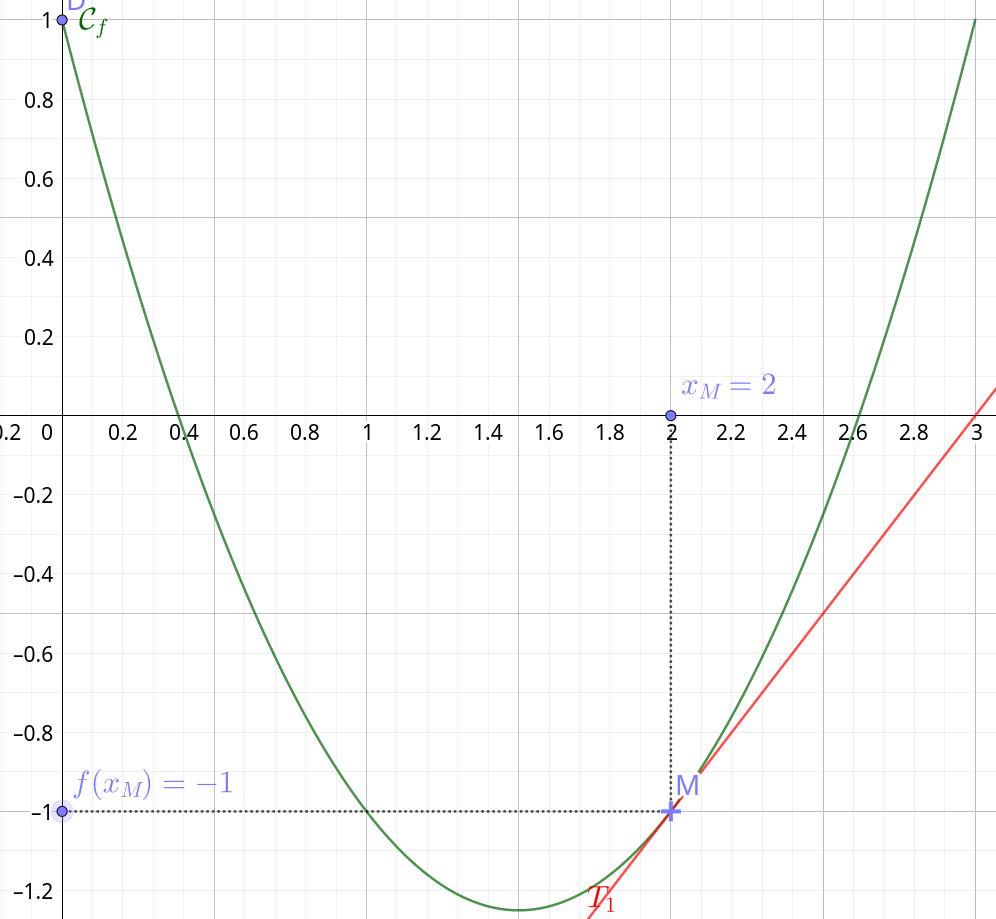
\includegraphics[width=.9\textwidth]{pics/graph2.png}
\caption{Graphe complété}
\label{graphe2}
\end{figure}

\question{}
$f'(x) = 2x-3$

\question{}
\og Algébriquement \fg{} signifie que cela doit être fait par le calcul et \emph{via} un raisonnement, par opposition à \og par lecture graphique \fg{}.

Il s'agit ici de chercher la (les) valeur(s) de $x$ pour lesquelles $f'(x) = 1$. En effet, on rappelle que le coefficient directeur de la tangente est le nombre dérivé. 
On cherche donc $x$ tel que:

$f'(x) = 1$

$\Leftrightarrow 2x-3 = 1$

$\Leftrightarrow x = 2$

$M \in \mathcal{C}_f$ et a pour abscisse 2. Il a donc pour coordonnées $(2;f(2))$.

$f(2) = -1$. 

On peut donc écrire $M(2;-1)$. 

\question{Voir figure \ref{graphe2}}

\question{} Il s'agit d'une droite, son équation est donc de la forme $y = ax+b$. Mais $a$ est déjà connu car il a été déterminé à la question 2: $a = 1$. On peut donc écrire $y = x+b$.

De plus, la tangente passe par le point $M(2;-1)$. On peut donc remplacer $x$ et $y$ par les coordonnées de $M$ et retrouver $b$:

$-1 = 2+b$

$\Leftrightarrow b = -3$

L'équation de la tangente est donc $y = x-3$.

\trait

\begin{center}
Fin.
\end{center}

\end{document}
